\begin{figure}[tbp]
\begin{center}
\includegraphics[width=0.4\textwidth]{z1z2powerden.eps}
\end{center}
\vspace{-0.7cm}
\caption{Density contrast power spectra $P_\delta$ at redshift 1 and 2.}
\label{fig:powerden}
\end{figure}
To explain the behavior of the cross correlation, we write Eq.(\ref{eq:ksz}) in Fourier space.

\begin{eqnarray}
    \Theta(\tilde{\bm{k}}_\perp)\equiv&\Theta&(\tilde{k}_x,\tilde{k}_y,0)\propto\int\, d^3k\delta(\tilde{\bm{k}}_\perp-\bm{k_\perp},k_\parallel) v_z(\bm{k})\nonumber\\
    \xrightarrow[region]{linear}&\int& d^3k\delta(\tilde{\bm{k}}_\perp-\bm{k_\perp},k_\parallel)\delta(\bm{k})\frac{k_z}{k^2}
%    =&\int&d^3\ln k\delta(\bm{k_\perp^{\prime}}-\bm{k_\perp},k_\parallel)\delta(\bm{k})\frac{k_z^2k_xk_y}{k^2}\nonumber
    \end{eqnarray}
\begin{eqnarray}
    \langle\Theta(\tilde{\bm{k}}_\perp)\Theta^{\ast}(\tilde{\bm{k}}_\perp)\rangle
    &\propto&\int \frac{d^3 \bm{k}}{(2\pi)^3}\frac{d^3 \bm{k^\prime}}{(2\pi)^3}
    \frac{k_z}{k^2}\frac{k^\prime_z}{k^{\prime2}}\\
    &&\langle \delta(\bm{k})\delta(\tilde{\bm{k}}_\perp-\bm{k})
    \delta^\ast(\bm{k^\prime})\delta^\ast(\tilde{\bm{k}}_\perp-\bm{k^\prime})\rangle
    \nonumber
\end{eqnarray}

The dominate term is 
$
    \langle \delta(\bm{k})\delta^\ast(\bm{k^\prime}) \rangle
    \langle \delta(\tilde{\bm{k}}_\perp-\bm{k})
    \delta^\ast(\tilde{\bm{k}}_\perp-\bm{k^\prime})\rangle
$ and 
$
    \langle \delta(\bm{k})
    \delta^\ast(\tilde{\bm{k}}_\perp-\bm{k^\prime})\rangle
    \langle \delta(\tilde{\bm{k}}_\perp-\bm{k})
    \delta^\ast(\bm{k^\prime}) \rangle
$
, hence, 
\begin{eqnarray}
    &&\langle\Theta(\tilde{\bm{k}}_\perp)\Theta^{\ast}(\tilde{\bm{k}}_\perp)\rangle
    \propto\int d^3 \bm{k}d^3 \bm{k^\prime}
    \frac{k_z}{k^2}\frac{k^\prime_z}{k^{\prime2}}
    \\
    &&P(k)P(\tilde{\bm{k}}_\perp-\bm{k})
    [\delta^D(\bm{k}-\bm{k^\prime})+\delta^D(\bm{k}+\bm{k^\prime}-\tilde{\bm{k}}_\perp)]\nonumber\\
%    &=&\int d^3 \bm{k}\, \frac{k_z^2}{k^2}
 %   P(k)P(\tilde{\bm{k}}_\perp-\bm{k})
%    (\frac{1}{k^2}-\frac{1}{|\tilde{\bm{k}}_\perp-\bm{k}|^2})\\
    &=&\int\, d^3\ln \bm{k}\, \frac{k_z^3k_xk_y}{k^2}
    P(k)P(\tilde{\bm{k}}_\perp-\bm{k})
    (\frac{1}{k^2}-\frac{1}{|\tilde{\bm{k}}_\perp-\bm{k}|^2})\nonumber
\end{eqnarray}

    We transform $dk\rightarrow d\ln k$ 
    to show the contributions from different k scales.
    Level of $P(k)$ can be seen in Fig.\ref{fig:powerden}

    For small $\tilde{k}_\perp^\prime \sim 0.01$ h/Mpc, 
    which corresponds to $\ell \sim 20-30$:
    
  Most $ (\frac{1}{k^2}-\frac{1}{|\tilde{\bm{k}}_\perp-\bm{k}|^2})
   \sim \frac{1}{k^3}$, 
   so we have $\frac{k_z^3k_xk_y}{k^5}$ which is scale invariant
   , and 
   $ P(k)\,P(\tilde{\bm{k}}_\perp-\bm{k})$
   reach peak at similar point with small k. 
   Therefore, main contribution of the powerspectrum is from large scale.
On the other hand, the fields after foreground substraction lack the part from small k, which causes the null correlation.

For large $\tilde{k}_\perp^\prime\sim 1$h/Mpc:

   $ (\frac{1}{k^2}-\frac{1}{|\tilde{\bm{k}}_\perp-\bm{k}|^2})
   \sim \frac{1}{k^2}$ or even $\sim \frac{1}{\tilde{k}_\perp^2}$
   so we have at least $\frac{k_z^3k_xk_y}{k^4}$, which prefers small scales.
   Moreover, $ P(k)\,P(\tilde{\bm{k}}_\perp-\bm{k})$
   no longer reach peak at similar point. 
Therefore, the importance of small k modes is attenuated, 
and the influence of foregrounds are reduced.

%Fig.\ref{fig:delta} is a set of plots that helps understand the behavior.
The reason why the correlation on redshift 2 is better is that 
the density contrast at redshift 1 is sharper than redshift 2, 
which exaggerates the contribution from small scales.
